%{Before beginning this investigation we must first know some important facts, formulae, laws and be familiar with the concepts that are to be incorporated in this investigation.}


        
\subsection{{Oxalic Acid}}
        
	{Oxalic Acid is an odorless, colorless white granular solid. It is synthesized from Acetic acid and is an organic compound belonging to the family of carboxylic acids. It is also a polar compound and is soluble in all polar solvents; Therefore it is an ideal solute to study the changes in the solubility in Alcohols with respect to temperature.}
		
\begin{figure}[H]
\centering
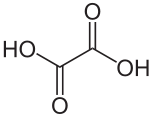
\includegraphics[width=5cm]{Oxacid.svg.png}
    		\caption{{2D chemic structure of the organic compound, Oxalic acid}}
\end{figure} 
            
\subsection{{Solubility in Alcohols}}
			
	{Alcohols are a class of polar compounds, therefore are perfectly soluble with polar solutes and solvents. As Oxalic Acid is polar, it is expected that all types of Alcohols would be perfect solvents for it.}
			
	{The property of Oxalic acid being polar makes it hydrophilic for Alcohol; and as a result it is also hypothesized that as the length of the alkyl chain increases, the non-polar part of the compound increases thus making the higher members of the Alcohol less polar, therefore decreasing its solubility with Oxalic Acid.}
			
%\subsection{{Stokes Law}}\label{slaw}
            


%\subsection{{Temperature dependence on density}}
            

            
%\subsection{{Computer Simulation Software}}
        

        
        


